%!TEX root = ../Thesis.tex
% Chapter Template

\chapter{Theory} % Main chapter title
\label{Theory} % Change X to a consecutive number; for referencing this chapter elsewhere, use \ref{ChapterX}
\lhead{Chapter \ref{Theory}. \emph{Theory}} % Change X to a consecutive number; this is for the header on each page - perhaps a shortened title

In this chapter the thesis will introduce the basic concept of clustering underpinning all clustering methods. It will formally define clustering and explain how the \STC algorithm fit into this definition. It will then move onto explaining the \STC algorithm itself and its different stages. It is in these sections that the parameters to be optimzed will be explained. The theory chapter will also go into some detail about the \CTC algorithm, a substantial modification of the original \STC algorithm. An investigation into performance measures used in information retrieval in general and clustering in particular will provide a foundation for how one can test the \STC and \CTC algorithms. The chapter will go shortly into two performance measurements suitable for \CTC. A short section about different corpora available for information retrieval research will also be presented.

In my thesis work a genetic approach to optimization of the parameters was tested. A section about the \GA will be provided to explain how this algorithm can be used for parameter optimization.

\section{Clustering and information retrieval}
\label{Clustering}
\citeauthor[][286]{Baeza-Yates2011a} defines text clustering as, ``\textit{[\dots] given a collection \(D\) of documents, a text clustering method automatically separates these documents into \(K\) clusters according to some predefined criteria}''. The variable \(K\) here refers to the number of clusters produced by the clustering algorithm given a document set. The variable \(D\) refers to the document set comprising the documents to be clustered. Given a document set \(D\) of size \(N\) a clustering algorithm might produce a cluster set where \(K \in \left\{1, .., 2^{N}-1\right\}\). In other words, a clustering algorithm might produce anywhere from a single cluster to as many clusters as there are document combinations.

The number of clusters variable \(K\) can either be pre-determined and given to the clustering algorithm as a variable as is the case with K-Mean Clustering. In other algorithms the \(K\) variable is undefined and varies according to different criteria such as the document collection size, the contents of the documents, the parameters given to the clustering algorithm etc.

It is not clear if the definition includes clustering algorithms that allow for overlapping clusters. \citeauthor{Baeza-Yates2011a} use the definition to describe agglomerative and partitional clustering. These two groups of clustering techniques do not create overlapping clusters, but the \STC and \CTC algorithms do. One could still argue that the \STC and \CTC algorithms conform to the definition of clustering proposed by \citeauthor{Baeza-Yates2011a}. Examples of other clustering algorithms that fall under this definition include the previously mentioned K-Mean algorithm and the Hierarchical Clustering algorithm.

\subsection{Suffix Trees and Suffix Tree Clustering}
The \STC algorithm was first introduced by \textcite{Oren1997} in the paper \citetitle{Oren1997}. This article discuss how suffix tree clustering can be used on search engine results to improve the results. Later an improved version of the algorithm was presented in the paper \citetitle{Oren1998} \cite{Oren1998}. In this later paper \citeauthor{Oren1998} describes the requirements for the \STC algorithm and the stages involved in \STC. They also compare the effectiveness (i.e. quality of results) of the algorithm compared to other clustering algorithms.

The \STC algorithm has three basic steps:
\begin{enumerate}
\item Document cleaning
\item Suffix tree and base cluster creation
\item Base cluster merging
\end{enumerate}

\subsubsection{Document Cleaning}

Document cleaning involves cleaning the strings representing each document. This is done by stemming each word, marking sentences, and removing non-word tokens such as HTML tags, numbers, and punctuation. The strings comprise the document snippets. Each snippet is a cleaned string from the original document. There are some possible parameters that can be identified here. For example, which parts of the documents should be extracted? Using more of the text document for snippet extraction gives the algorithm more data to work with which could yield more accurate results. There is also the question of which parts of the documents that are the best signifier of the document's content. For news documents a parameter could determine which parts of the document to include, such as titles, headings, (image) captions, article introductions, main text and so forth. Two other possible parameters that have not been investigated are possible stemming techniques (lemmatisation vs. stemming) and different stop word lists.

\subsubsection{Suffix Tree and Base Cluster Creation}

To make the concept Suffix Trees a bit clearer a short explanation of the trie data structure and suffixes will be provided.

The \STC algorithm use a trie data structure. Trie data structures are trees that store sets of strings. Figure~\ref{fig:triedatastructure} shows an example of a trie data structure containing the words mouse, moose, muse, nonse, and nose.

\begin{figure}[!ht]

   \Tree[.*
   			[.m 
   				[.o 
   					[.o [.s [.e ]]]
   					[.u [.s [.e ]]]
   				]
   				[.u [.s [.e ]]]
   			]
   			[.n 
   				[.o [.n [.s [.e ]
   						]
   					]
   					[.s 
   						[.e ]
   					]
   				]
   			]
   		]

  \caption{An example trie data structure}
  \label{fig:triedatastructure}
\end{figure}

A trie data structure can also be used as search tree, which gives it certain properties. A search tree is a multi-way tree \footnote{\url{http://faculty.cs.niu.edu/~freedman/340/340notes/340multi.htm}}. What this means is that in a multi-way tree on the order of 5, each node can have up to five children. Such a tree would be called a five-way tree. In a search tree each child node is ordered by some criteria, for example by their alphabetical order. This makes it possible to retrieve any string encoded within the tree in time proportional to the string's length, \cite{Baeza-Yates2011c}.

\citeauthor{Baeza-Yates2011c} also compare the compact trie structure to a deterministic finite automaton (DFA). The DFA will not be described in detail here, but it does offer an interesting and perhaps enlightening background for the structure of suffix trie data structures. Essentially a DFA graphs states and transitions between them in a deterministic and finite manner. For text matching a DFA is used to represent string patterns, regular expressions, that can be matched against text. A DFA needs to have a start state and a finite state.

A suffix trie is a graph over a collection of strings where the root represents the initial state (no match), and each leaf node denotes a final state (match with a specific suffix). Each edge that makes up the path from the root of the suffix trie to a leaf node is labeled with a letter from that suffix. Suffixes that start with the same letters will use the same edges. In essence the suffix trie forms a search tree over all suffixes expanded from a list of strings. So what is a suffix?

In context of a term \(T = [c_{1}, ..., c_{n}]\) a suffix is a sub-term \(S = [c[n-m], \dots, c[n]]\) where \(0 \le m < n\). For example the suffixes of the term ``suffix'' are
\begin{inparaenum}[\itshape 1\upshape)]
\item suffix;
\item uffix;
\item ffix;
\item fix;
\item ix; and
\item x
\end{inparaenum}.

\cite{Oren1998} treat documents as a collection of snippets where each snippet is a normalized sentence from a document. Each snippet contains a sequence of words. The \STC algorithm extracts its suffixes from phrases (snippets) rather than single terms. A suffix in this context would thus be defined as all the sub-phrases of a given phrase. Following the same rules as apply for the example above the phrase ``clustering is fun'' therefore has the following suffixes:
\begin{inparaenum}[\itshape 1\upshape)]
\item clustering is fun,
\item is fun, and
\item fun
\end{inparaenum}.

By combining the concepts of suffixes and trie structures one can build a suffix tree. \cite{Oren1998} formally define a suffix tree of string \textit{S} with the following requirements:
\begin{itemize}
\item Suffix trees are rooted and directed.
\item All internal nodes have at least two children.
\item Each edge is labeled with a non-empty substring of \textit{S}.
\item A node's label is defined as the concatenated labels of the nodes in the path from the root node to the given node.
\item Edges from the same node can not have the same edge-labels (sub-phrases)
\item For each suffix of the string \textit{S} there is a suffix node which represents that suffix.
\end{itemize}

Following these requirements one can understand a suffix tree as a tree where edges represent suffixes of or whole phrases. Each node pointed to by an edge represents the collection of documents or sources from which the suffix has been collected. A leaf node is the collection of all documents that contain that specific phrase or sub-phrase, and each internal node is a phrase cluster made up of all documents sharing the sub-phrase given by the edge label.

An example of a suffix tree can be seen in Figure~\ref{fig:suffixtree}. Here three phrases each comprising a document are split into suffixes and then put into the suffix tree structure. As an example one can see that the two phrases
\begin{inparaenum}[\itshape 1\upshape)]
\item ``cat ate cheese'' and
\item ``cat ate mouse too''
\end{inparaenum}
share the phrase ``cat ate''. This is represented in the graph (Figure~\ref{fig:suffixtree}) by node \textit{a} which contains pointers to the first suffix of both phrase 1 and phrase 2.

\begin{figure}[!ht]
  \begin{center}
    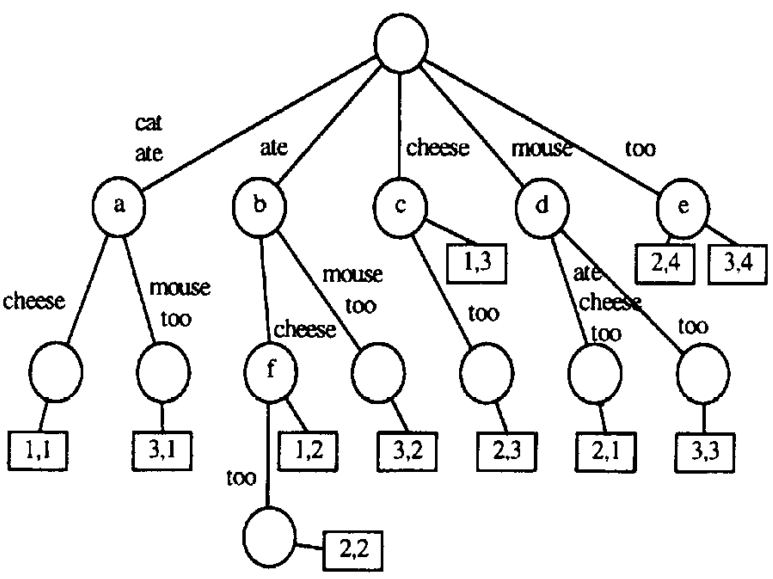
\includegraphics[totalheight=0.3\textheight]{Figures/suffixtree}
  \end{center}
  \caption{A suffix tree generated from the strings “cat ate cheese”, “mouse ate cheese too” and “cat ate mouse too”. From \citetitle{Oren1998} \protect \cite[][48]{Oren1998}}
  \label{fig:suffixtree}
\end{figure}

Each internal node is a phrase cluster made up of all the documents that share that phrase (i.e the union of the documents in its descendant nodes). Each node makes up a base cluster \cite{Oren1998}. The base clusters are scored according to the scoring function: 
%Math formula
\begin{displaymath}s(B) = 
\vert B \vert \cdot f(P)
\end{displaymath} 
where \(\vert B \vert\) 
is the number of documents in the cluster \(B\) and  \(f(P)\) is a function on the length of the cluster phrase \(P\) (excluding stop words) which penalizes short phrases (\( P < 2\)), gives a linear score for regular phrases (\(P = {2,\dots,6}\)) and a constant score to longer phrases (\( P > 6\)). Clusters with many documents and/or long phrases receive higher scores than clusters with few documents and/or short phrases. A promising parameter identified in this step would be the score-threshold used by the \(f(P)\)-function. The scoring-threshold determines which of the terms in a phrase that contributes to that phrase's length. If a term is contained within 3 or less documents or more than 40\% of the documents in the collection the term receives a score of zero and does not contribute to the phrase's length. This could influence the scores of base clusters as some base clusters could become longer or shorter. The base cluster score is used to sort the base clusters for the final step in the \STC algorithm.

\subsubsection{Base Cluster Merging}
Base cluster merging is the final step in the \STC algorithm and is an improvement of the original algorithm. \citeauthor{Oren1998} note that,
\begin{quote}
Documents may share more than one phrase. As a result, the document sets of distinct base clusters may overlap and may even be identical. To avoid the proliferation of nearly identical clusters, the third step of the algorithm merges base clusters with a high overlap in their document sets [\dots] \cite[][3]{Oren1998}
\end{quote}

Base clusters are merged based on their similarity. \citeauthor{Oren1998} use a similarity measure based on a binary relationship between the number of shared documents in the two base clusters. This similarity measure will hereforth be reffered to as ``Etzioni similarity''. Given two base clusters \(B_m\) and \(B_n\) ``Etzioni similarity'' is formally defined as 

\begin{displaymath} 
S_{m}(B_{m},B_{n}) = 
\frac{\vert B_{m} \cap B_{n} \vert} {\vert B_{m} \vert}
\end{displaymath}

\begin{displaymath} 
S_{n}(B_{m},B_{n}) = 
\frac{\vert B_{m} \cap B_{n} \vert} {\vert B_{n} \vert}
\end{displaymath}

Iff \(S_{m} > 0.5\) and \(S_{n} > 0.5 \) then the ``Etzioni similarity'' of the two clusters \(m\) and \(n\) is equal to 1. This measure should not be confused with the Jaccard similarity coefficient which is expressed as 

\begin{math}
\frac{\vert X \cap Y \vert} {\vert X \cup Y \vert}
\end{math}, where the similarity can vary between zero if there are no common elements in set \(X\) and \(Y\) and one if the two sets have all elements in common, \cite{VanRijsbergen1979}. The ``Jaccard similarity'' of the two base clusters can be expressed as

\begin{displaymath} 
S(B_{m}, B_{n}) = 
\frac{\vert B_{m} \cap B_{n} \vert} {\vert B_{m} \cup B_{n} \vert}.
\end{displaymath}

Iff the ``Jaccard similarity'' is greater than 0.5 are the two base clusters considered equal. The Jaccard similarity coefficient is a stricter measure. This is true because \(\vert B_{m} \cup B_{n} \vert\ \geq \vert B_{n} \vert\) and \(\vert B_{m} \cup B_{n} \vert\ \geq \vert B_{m} \vert\). Jaccard similarity thus imply Etzioni similarity, but Etzioni similarity does not imply Jaccard Similarity.

All base cluster pairs with a similarity of 1 is connected in a base cluster graph. This results in a set of connected components in the graph. Each connected component is considered a cluster in the final clustering result. In this last step, two parameters can be identified. One could adjust the number of base clusters used to create the final clusters. The lowest scoring base clusters might not be relevant for the final results as the documents in these clusters share few of their phrases with each-other. On the other hand it might hurt the results if the algorithm use too few of the base clusters resulting in a lower number of merged clusters, or even less accurate merged clusters.

It is also possible to adjust the similarity threshold used by the Jaccard coefficient, or use another similarity measure all together. One such similarity measure is the cosine similarity measure that can be used when documents are represented in a vector space model. The vector space model is most often used with the bag of words model where each vector consist of single terms. The vector space model could also be used with phrases as investigated by \cite{Chim2007}.

The cosine similarity formula returns a value between -1 and 1, where -1 denotes that the vectors being compared are completely dissimilar, 1 that they are identical, and 0 that they are somewhere in between. The cosine similarity value can easily be applied as a similarity measure when combining clusters.

How exactly is the cosine similarity of two documents computed? Usually the cosine similarity is computed using the vector space model where each vector feature is represented with a weight value, \cite{Manning2009a}. It is not uncommon to use a tf-idf weighing scheme. In this model there are some key elements. There is a document \textit{corpus} consisting of \(N\) number of text documents. From this corpus one can compute a \textit{dictionary} comprising all the terms in the corpus and their frequency. A term's corpus frequency is thus the number of times it occurs in the corpus. The \textit{term frequency} (tf) of a term is the number of times it occurs in a document. The \textit{document frequency} (df) of a term is the number of documents it occurs in. A terms weight can be measured by it's tf-idf score \cite{Manning2009a}. The tf-idf score of a given term can be calculated given the functions:


\begin{displaymath}
idf{t} = log \frac{N}{df_{t}} 
\end{displaymath}

\begin{displaymath}
tf-idf_{t,d} = tf * idf
\end{displaymath}

The inverse document frequency measures the relative uniqueness of a term in the collection by giving terms occurring in fewer documents higher scores than those occuring in most documents. Given a document a term will then receive a high tf-idf weight if it occurs frequently in that document, but in few documents in the collection. Converesly, if the term occurs a small amount of times in a document, but in all documents it will be given a very low weight.

The cosine similarity of two documents are found by calculating the dot product of their two magnitude vectors and then dividing that by the product of their Euclidian length to length-normalize the result \cite{Manning2009a}. It can be expressed mathematically as follows:

\begin{displaymath}
sim(d1, d2) = \frac{\vec{V}(d1) * \vec{V}(d2)}
{\sqrt{\sum_{i = 1}^M\vec{v}_{i}^2(d1)} * \sqrt{\sum_{i = 1}^M\vec{v}_{i}^2(d2)}}
\end{displaymath}

The vector representation of each document consist of one component for each term in the corpus dictionary. The components can be derived by different means, but it is common to use the tf-idf score of a term as components for a document vector. The vector representation \(\vec{V}(d)\) is thus the tf-idf score for each term \(t\) in document \(d\) given a corpus. The tf-idf weighing scheme and cosine similarity function can be adapted to work within the base cluster context. This will be explained later in Chapter~\ref{DesignDevelopment}.

\subsection{Compact Trie Clustering}
The \CTC algorithm is a modified version of the \STC algorithm authored by \cite{Moe2013}. It is a generalization of the \STC algorithm. \cite{Moe2013} modified the algorithm to use n-grams in the snippet expansion phase, as well as adding functions for dropping base clusters containing only one document and clusters with one word labels.

 A n-gram is a subsequence of \(k\) number of characters in a token. In the token ``mouse'' all the 3-grams would be: \$mo, mou, ous, use, \$se, \cite{Manning2009}. A n-gram can also be applied on phrases. the k-grams of a phrase is all the subsequences of \(k\) words occurring in that phrase. The 3-grams of the phrase ``mouse ate cheese too'' is
\begin{inparaenum}[(1)] 
    \item mouse ate cheese
    \item ate cheese too
\end{inparaenum}.

\subsection{Performance measures}
My thesis will evaluate the performance of the clustering algorithm in two ways. First, a measurement of the performance will be used as a fitness-function in the \GA. Second, the performance of the system will be evaluated using unoptimized and optimized parameters as part of an experiment that will be described in more detail later. To measure the performance of the \CTC algorithm it is necessary to have a clear definition of performance.

\cite[][131]{Baeza-Yates2011b} define retrieval evaluation as a \begin{quote} 
[\dots] process of systematically associating a quantitative metric to the results produced by an IR system in response to a set of user queries. This metric should be directly associated with the relevance of the results to the user. A common approach to compute such a metric is to compare the results produced by the system with results suggested by humans for that same set of queries.
\end{quote}
Retrieval evaluation thus requires a ground truth, i.e. a human judgment of relevance for a set of documents for a given query, or in context of text clustering a human defined classification of a document.

There are several metrics for results in information retrieval. Two common, and among the most basic, are \textit{precision} and \textit{recall}. \cite{Sebastiani2002,Baeza-Yates2011a} provide formulas for calculating precision and recall for text classifiers.

Precision with regards to a \(class\) can be calculated with the formula:
\begin{displaymath}
Precision = 
\frac{TP}{TP + FP}
\end{displaymath}
where \(TP\) (i.e. True Positive) is the number of documents correctly assigned to the \(class\) and \(FP\) (i.e. False Positive) is the number of documents falsely assigned to the \(class\). Precision thus express the ratio of correctly classified documents to wrongly classified documents. A precision of 1 means there are no wrongly classified documents for the \(class\).

Recall with regards to a \(class\) can be calculated with the formula: 
\begin{displaymath}
Recall = 
\frac{TP}{TP + FN}
\end{displaymath}
where \(FN\) (i.e. False Negatives) is the number of documents wrongly not assigned to the \(class\). Recall express the number of documents correctly assigned to the \(class\) to the number of documents assigned to the \(class\) in total. A value of 1 signifies that all documents were correctfully assigned to the \(class\).

This notion of precision and recall works with a binary notion of relevance for the relationship between a document and class. A document either is, or is not, a member of a given class. The ``Klimauken'' corpus use a different definition of relevance where clusters might overlap. These definitions of precision and recall can therefore not be applied when testing the \CTC algorithm with this corpus.

% An article by \cite{Yang1999} describe a comparative evaluation of different text classifiers that measure how well the classifiers perform on different versions of the Reuters corpus. The article also provides formulas for precision, recall and F-Measure in context of text classifiers. They also describe how the 11-point system can be used to find the overall performance of the system.


% \subsection{Available corpora}
% There are different corpora used in information retrieval research. TREC describes a number of corpora, but most of these are created for the benefit of search algorithms and are not very suitable for testing clustering algorithms. \citeauthor{Baeza-Yates2011a} describe some of the most used benchmark collections in text classification research: Reuters-21578, RCV: Reuters Corpus Volumes, OHSUMED reference collection, and 20 NewsGroups. Some of them are desribed in greater detail below.

% Reuters, an international news agency has made several corpora that are available trough different sources. One Reuters corpus that has been much used in the text classification community is the \textit{Reuters 21578} corpus \cite{Lewis2004a}. The documents in this collection was collected from documents appearing on the Reuters newswire in 1987. It was assembled and categorized by personnel from Reuters and Carnegie Group in 1987. The corpus thus resembles that used in the ``Recycling of news in the news papers 1999 - 2000'' research project.

% Reuters have since made a new corpus that is likely to replace the Reuters 21578 corpus. This new corpus is divided into three volumes RCV1, RCV2 and TRC2. The first two volumes contain news stories from 96 - 97, and the last volume contains news stories from 08 to 09. RCV1 and TRC2 contain English news stories only, while RCV2 is multilingual \cite{NationalInstituteofStandardsandTechnology2004}. An article on the use of the RCV1 corpus provide more details about how the data set can be used in evaluation of text categorization systems. ``\textit{Reuters CorpusVolume I (RCV1) is an archive of over 800,000 manually categorized newswire stories recently made available by Reuters, Ltd. for research purposes. Use of this data for research on text categorization requires a detailed understanding of the real world constraints under which the data was produced.}'' \cite{Lewis2004}. 

% Because the thesis work were performed under time constraints the main focus of the thesis remained on the ``Klimauken'' corpus. Further research into the optimization problem would however likely include these other corpora.

\section{Genetic Algorithms}
\label{GeneticAlgorithm}
In the book \citetitle{Haupt2004} by \cite{Haupt2004} optimization is defined as ``\textit{[\dots] the process of adjusting the inputs to or characteristics of a device, mathematical process, or experiment to find the minimum or maximum output or result }''. Variables are provided as input to the optimization problem, the output is the cost of the given input. In genetic algorithms the cost is also known as fitness. Examples of local optimization algorithms are Exhaustive Search, Nelder-Mead Downhill Simplex Method, Hill Climbing and so forth. These algorithms are most suited to finding local optimums (lowest cost) and will as such not be considered in this thesis work, \cite{Haupt2004}.

Because the cost surface of the optimization problem for the optimal \CTC cluster parameters features several cost tops and bottoms it is necessary to use global optimization algorithms. Two examples of these are the Genetic Algorithm and the Swarm Optimization algorithm. This thesis will focus on the Genetic Algorithm because of time constraints and familiarity with the algorithm.

The genetic algorithm is inspired by natural selection and genetics. It is used to solve search and optimization problems. According to \citeauthor[23]{Haupt2004} the genetic algorithm has several advantages namely that it:
\begin{inparaenum}[\itshape 1\upshape)]
\item Optimizes with continuous or discrete variables;
\item Searches a wide sampling of the cost surface simultaneously;
\item Works on optimization problems with complex cost surfaces and
\item Provides a list of optimum values (the final population) 
\end{inparaenum}

The Genetic Algorithm can be divided into two main categories, binary and literal values. Binary genetic algorithms use binary code as the genetic markup of the chromosomes whilst literal value genetic algorithms instead use literal values such as numbers and characters. \citeauthor{Haupt2004a} use the binary algorithm as a base to describe genetic algorithms. A \textit{chromosome} is a vector of variables or parameters: \(Chromosome = [p_{1},p_{2},p_{3},\dots,p_{n}]\). The fitness-function takes as input the \textit{chromosome} and outputs the fitness of that chromosome according to some fitness evaluation function. Each parameter \(p_{n}\) represents a \textit{gene}, and can be encoded as a binary sequence or as a literal value. \citeauthor[p. 93]{Brownlee2011} note that, ``\textit{Problem specific representations and customized genetic operators should be adopted, incorporating as much prior information about the problem domain as possible}''. Both because it would be difficult to encode the parameter sets of the \CTC algorithm and to retain the beneficial values in a binary system, it seems literal values would be better suited for the optimization problem.

\begin{figure}[!h]
  \begin{center}
    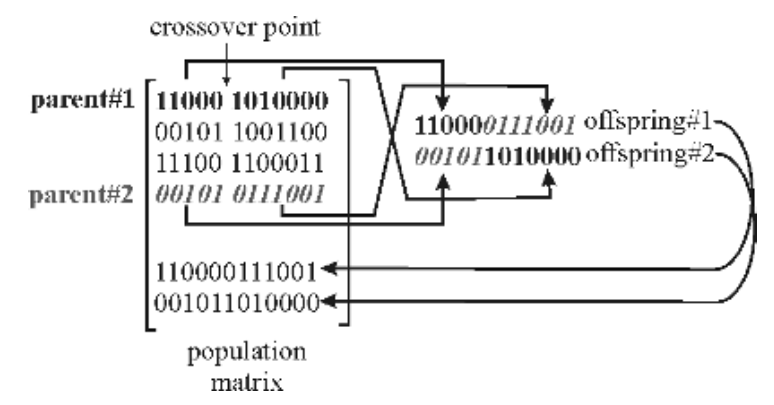
\includegraphics[totalheight=0.175\textheight]{figures/crossover}
  \end{center}
  \caption{Two parent chromosomes produce two offspring. The offspring chromosomes inherit the genes according to the position of the crossover point. From The Binary Genetic Algorithm \protect \cite[p. 42]{Haupt2004a}.}
  \label{fig:crossover}
\end{figure}

The Genetic Algorithm can be divided into some simple steps:
\begin{inparaenum}[\itshape 1\upshape)]
\item Create an initial population;
\item Sort population and drop part of the population according to fitness;
\item Select pairs of chromosomes for mating;
\item Do crossover mating for each pair;
\item Insert new child chromosomes into population;
\item Mutate a random gene in a random selection of chromosomes;
\item Sort population according to fitness;
\item See if chromosomes have converged, if not go back to step 2, and
\item Return the resulting chromosomes
\end{inparaenum}

Initially the genetic algorithm starts with a set of chromosomes, a \textit{population}. The population is generated by setting random values for each gene \cite{Haupt2004a,Negnevitsky2002,Goldberg1989}. Each gene is assigned a fitness based on a predefined fitness function. In the pseudo implementation presented by \citeauthor{Haupt2004a} the top \(N\) chromosomes are deemed fit for survival and the rest are discarded.

The algorithm then selects pairs of chromosomes for the \textit{mating process} according to their fitness. There are several different selection techniques such as roulette-wheel weighting, random pairing, and tournament selection, \cite{Haupt2004a}. Which one works best depends on the optimization problem. The mating process generally involves generating two offspring from two parents. The algorithm selects at random a crossover point at some position in the chromosomes' gene sequence and then combines the start and end segments of the two parents as described in Figure~\ref{fig:crossover}.

To avoid early \textit{convergence} in the population the \GA mutates a random selection of offspring chromosomes by mutating a randomly selected gene. The number of chromosomes and genes mutated depends on the \textit{mutation rate}. \cite{Goldberg1989,Negnevitsky2002} inform that a mutation rate between 0.001 and 0.01 is normal. The mating and mutation steps reiterates till some cut-off or convergence criteria is met.

\section{Related Work}
\label{RelatedWork}
In \citetitle{Zakos2005} a paper by \citeauthor{Zakos2005}, the authors discuss how the Genetic Algorithm can be used to optimize an Information Retrieval technique called Context Matching. The goal of their work," \textit{{\dots} is to investigate the use of an evolutionary algorithm for the optimization of context matching parameters and compare its performance to an iterative technique that exhaustively explores combinations of parameters}" \cite[582]{Zakos2005}. Their research showed that the Genetic Algorithm can be used to effectively find optimal parameters for context matching. They also noted how the Genetic Algorithm converged on some parameters (linear distance) and showed that some parameter values were viable.

A similar goal is pursued for the Okapi system in a paper written by \cite{Chuan2003}.The Okapi system is a document search algorithm that implements a probabilistic model for ranking of results. The system implements the BM2500 weighting function which has a number of parameters that influence the ranking result. In an article by \cite{Chuan2003} it is shown how their genetic algorithm improves the precision of the top ten results as well as the mean average precision of the results compared to experimental results.

% \cite{gulla2008contextualized} discuss how clustering (specifically Suffix Tree Clustering) can be used to help users browse trough large result sets in exploratory web search. The authors present a search engine, HOBSearch, which implements clustering of search results based on the Suffix Tree Algorithm. \citeauthor[21]{gulla2008contextualized} conclude that, ``\textit{The evaluation indicates that the resulting clusters are coherent and that clustering several hundred documents on the fly is feasible.}''.

In a paper by \cite{Chim2007} a new clustering algorithm combining the \STC and vector space-based Hierarchical Clustering algorithm is proposed. This algorithm use the Suffix Trie data structure to build a collection of phrase-source pairs, and then insert the pairs into a hierarchy using the standard Hierarchical Clustering algorithm. The improved algorithm is shown to have improved performance. They also detail how they implement the F-measure in their evaluation of the clustering algorithm. This algorithm was later compared to other clustering algorithms in \citetitle{Chim2008}, \cite{Chim2008}. In this thesis work the focus will be on improving the \CTC algorithm. The paper did however inspire a new vector based similarity measure for base cluster merging, \cite{Moe2013}.